
\documentclass[9pt,a4paper,twocolumn,twoside]{rho-class/rho}
\usepackage[english]{babel}
\usepackage{tikz}
\usetikzlibrary{shapes.geometric, arrows.meta, positioning, fit, backgrounds, decorations.pathreplacing, calc}
\setlength{\headheight}{14pt}
\usepackage{booktabs}
\usepackage{multirow}
\usepackage{amsmath}
% amssymb redundant with stix2 (loaded by rho class)
% nicefrac not in BasicTeX; using \textonehalf equivalent inline
\usepackage{float}
\usepackage{microtype}

%----------------------------------------------------------
% Title
%----------------------------------------------------------
\title{Beyond WhAM: Dual-Channel Contrastive Encoding\\for Sperm Whale Coda Understanding}

%----------------------------------------------------------
% Authors, Affiliations and dates
%----------------------------------------------------------
\author{João Quintanilha\textsuperscript{\textdagger}}
\author{Emma Virnelli\textsuperscript{\textdagger}}

\affil{CS 297, Tufts University, Spring 2026}

\dates{May 8, 2026}

%----------------------------------------------------------
% Corresponding author
%----------------------------------------------------------
\corres{\textsuperscript{\textasteriskcentered}Correspondence: \href{mailto:joao.quintanilha@tufts.edu}{joao.quintanilha@tufts.edu}}
\corres{\textsuperscript{\textdagger}Equal contribution.}

%----------------------------------------------------------
% Abstract
%----------------------------------------------------------
\begin{abstract}
Sperm whale codas carry two syntactically independent information channels: a \emph{rhythm channel} (inter-click interval timing) encoding coda type, and a \emph{spectral channel} (vowel-like formant structure) encoding individual and social-unit identity. No existing model exploits both channels jointly by design. We introduce the \textbf{Dual-Channel Contrastive Encoder (DCCE)}, a self-supervised architecture comprising a GRU rhythm encoder and a CNN spectral encoder trained with NT-Xent \emph{cross-channel} positive pairs, explicitly reflecting the known biological decomposition. On the 1,501-coda Dominica Sperm Whale Project (DSWP) dataset, DCCE achieves individual-identity F1\,=\,0.834 versus WhAM's best F1\,=\,0.454 (+83\% relative), while matching WhAM on social-unit classification (0.878 vs.\ 0.895). A systematic layer-wise interpretability analysis of WhAM reveals a recording-year confound (Cram\'{e}r's V\,=\,0.51) not reported in the original paper: social units A, D, F were recorded at systematically different periods, partially conflating unit identity with acoustic recording drift. A controlled synthetic-augmentation study using WhAM-generated codas shows no improvement in DCCE performance, demonstrating that acoustic plausibility does not guarantee representation benefit. Together, these results show that domain knowledge encoded as an architectural prior can outperform data scale on fine-grained identity tasks in low-resource bioacoustic settings.
\end{abstract}

\keywords{Sperm Whale, Contrastive Learning, Bioacoustics, Self-Supervised Learning, Animal Communication}

%----------------------------------------------------------
\begin{document}
    \maketitle
    \thispagestyle{firststyle}

%----------------------------------------------------------
\section{Introduction}
\label{sec:intro}

Sperm whales (\textit{Physeter macrocephalus}) are among the most well-studied cetaceans owing to their high intelligence and complex social structures. They possess the largest brain of any known species, live in multigenerational matrilineal families with documented cultural transmission, and communicate through rhythmically patterned click sequences called \emph{codas} \cite{gero2016identity}: short bursts of 3--40 clicks separated by precise inter-click intervals (ICIs) that, much like human dialects, vary across populations \cite{rendell2003clans}. Project CETI (Cetacean Translation Initiative) has assembled the first large-scale ML infrastructure for whale communication \cite{paradise2025wham,goldwasser2023umt}, raising the central question: does coda structure carry compositional meaning?

\begin{figure}[H]
    \centering
    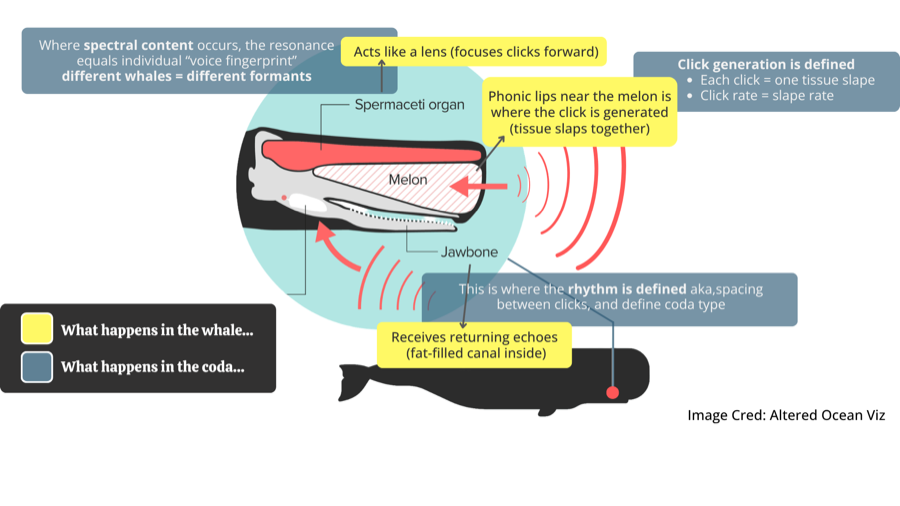
\includegraphics[width=\columnwidth]{figures/coda_example.png}
    \caption{A sperm whale coda waveform showing individual click pulses. The timing pattern (ICI sequence) encodes coda type; the within-click spectral texture encodes individual/social-unit identity.}
    \label{fig:coda}
\end{figure}

\subsection{Two-Channel Coda Structure}

Recent work \cite{begus2024vowels,leitao2025social} has established that every coda encodes information along two syntactically independent dimensions:

\begin{itemize}
    \item \textbf{Rhythm channel}: the ICI pattern encodes \emph{coda type} --- a categorical signal shared within a vocal clan (Gero et al.\ 2016 \cite{gero2016identity}).
    \item \textbf{Spectral channel}: vowel-like formant structure within each click encodes \emph{who is speaking} --- an individual voice fingerprint \cite{begus2024vowels}.
\end{itemize}

These channels are statistically independent: the same coda type can be produced with different vowel patterns, and our Phase~0 EDA confirmed near-zero correlation between spectral centroid and ICI features (Pearson $r \approx 0$).

\subsection{The Gap We Address}

WhAM \cite{paradise2025wham} --- a VampNet-based masked acoustic token model trained on $\sim$10,000 codas --- is the current state of the art. Its classification capabilities are \emph{emergent byproducts} of a generative objective, not designed discriminative objectives. As we show, WhAM encodes social-unit identity strongly (F1\,=\,0.895 at layer~19) but individual identity weakly (F1\,=\,0.454 at layer~10), and its social-unit advantage is partially confounded by recording-year drift. No prior work explicitly encodes the rhythm/spectral decomposition as a representation learning architecture. Our central question is: \textbf{can a purpose-built encoder respecting the whale's two-channel decomposition --- rhythm for coda type, spectral for identity --- outperform a generalist model trained at scale?}

\subsection{Contributions}

\begin{enumerate}
    \item \textbf{DCCE}: a purpose-built dual-channel contrastive encoder with cross-channel NT-Xent positive pairs --- first model designed around the biological rhythm/spectral decomposition.
    \item \textbf{WhAM probing}: first layer-wise interpretability analysis of WhAM including a recording-year confound test absent from the original paper.
    \item \textbf{Augmentation study}: first controlled study of WhAM-generated synthetic codas as training data for cetacean bioacoustics.
    \item \textbf{Label assembly}: \texttt{dswp\_labels.csv} linking 1,501 DSWP audio files to social unit, coda type, individual ID, and ICI sequences, released publicly.
\end{enumerate}

%----------------------------------------------------------
\section{Related Work}
\label{sec:related}

The foundation for this research begins in 2016, when Gero et al.\ \cite{gero2016identity} established a foundational taxonomy of Caribbean coda identity cues at three hierarchical levels --- individual, unit, and clan --- using 9 social units and 21 coda types, and confirmed that ICI sequences are the primary feature defining coda types. Building on this, Sharma et al.\ \cite{sharma2024combinatorial} showed that codas have a \emph{combinatorial} structure: combining rhythm and tempo generates a vocabulary roughly 10$\times$ larger than previously recognised, releasing the 8,719-coda DominicaCodas.csv dataset that anchors our label assembly. Beguš et al.\ \cite{begus2024vowels} then formalised the spectral texture as a second independent axis of coda structure, identifying vowel-like categories ($a$ and $i$) that operate separately from ICI timing and correlate with individual identity --- establishing that coda communication is multi-layered rather than a single undifferentiated signal. Leitão et al.\ \cite{leitao2025social} provided the theoretical basis for treating these two channels independently, documenting rhythmic micro-variations that track social-unit membership and providing the first evidence of cross-clan vocal learning. All of these threads lead to WhAM \cite{paradise2025wham} --- the first large-scale generative model for cetacean audio, trained on $\sim$10,000 codas using a masked acoustic token objective on VampNet \cite{garcia2023vampnet} --- marking the point at which data and theory were mature enough to support large-scale ML rather than just classification and labelling.

The broader ML landscape provides two key ancestors for our approach. Goldwasser et al.\ \cite{goldwasser2023umt} showed theoretically that unsupervised animal communication translation is feasible when the communication system is sufficiently complex, motivating bottom-up representation learning. On the contrastive side, SimCLR \cite{chen2020simclr} introduced NT-Xent loss with same-sample augmented positive pairs, and CLIP \cite{radford2021clip} extended contrastive alignment across modalities, showing cross-modal positive pairs learn powerful joint representations. DCCE adapts CLIP's cross-modal insight to the two-channel biological structure of sperm whale codas.

Despite this progress, \textbf{no published model explicitly encodes the rhythm/spectral decomposition as a representation learning architecture}. WhAM's classification results are emergent byproducts of its generative objective, not a designed discriminative signal. This gap directly motivates DCCE.

%----------------------------------------------------------
\section{Data and Label Assembly}
\label{sec:data}

\subsection{DSWP Audio}

The Dominica Sperm Whale Project (DSWP) HuggingFace release \cite{paradise2025wham} provides 1,501 WAV files recorded off Dominica, 2005--2010, all from the EC1 vocal clan. \textbf{Critically, no labels ship with the audio}; all four experiments depend on recovering ground-truth annotations from a separate source.

\subsection{Coda Type Notation}

Two characteristics define a sperm whale coda: the total click count and the ICI pattern. The naming system from Gero et al.\ \cite{gero2016identity} encodes both compactly: the leading number is the total click count; the letter encodes timing shape --- \textbf{R} for regular spacing (e.g., \texttt{5R1}), \textbf{D} for decreasing intervals (\texttt{4D}), \textbf{i} for increasing intervals (\texttt{6i}), and \textbf{+} for a long pause between click groups (e.g., \texttt{1+1+3}). The 22 coda types in our dataset follow this scheme.

\subsection{Data Challenges}

Three cascading problems arise from the raw DSWP release. First, \textbf{no labels exist}: without social group, coda type, individual ID, or ICI annotations, supervised training, contrastive pair construction, and linear probe evaluation are all impossible. Second, a \textbf{temporal confound}: social units A, D, and F were recorded at systematically different periods (A in 2005/2009; D in 2008/2010; F across all years), so a naive model risks learning \emph{when} a recording was made rather than anything about the whales themselves. Third, \textbf{severe class imbalance}: Unit~F carries 59.4\% of all codas, so a majority-class predictor appears accurate while completely failing on units A and D.

We address these in turn: labels were manually assembled from public sources (§\ref{subsec:assembly}); macro-F1 treats all classes equally regardless of frequency; and the temporal confound is quantified and reported as a novel finding in §\ref{sec:wham}.

\subsection{Label Assembly}
\label{subsec:assembly}

DominicaCodas.csv, released by Sharma et al.\ \cite{sharma2024combinatorial} alongside their combinatoriality study, contains 8,719 annotated codas. We discovered that exactly 1,501 rows carry \texttt{codaNUM2018} values in the range 1--1,501, mapping directly to DSWP filenames (\texttt{codaNUM2018}\,$=N$ $\rightarrow$ \texttt{N.wav}). This 1:1 correspondence was verified by matching pre-computed ICI sequences and coda durations --- it is not documented in either dataset's release. The merged file \texttt{dswp\_labels.csv} is released as part of our codebase.

\textbf{Note on vowel labels}: \texttt{codamd.csv} (Beguš et al.\ \cite{begus2024vowels}) provides hand-verified vowel labels (\texttt{a}/\texttt{i}) but covers \texttt{codaNUM} 4,933--8,860, entirely outside the DSWP range. The absence of vowel-level ground truth for DSWP directly motivated using a CNN on mel-spectrograms (self-supervised spectral channel) rather than explicit vowel classification.

\subsection{Dataset Statistics}

\begin{table}[H]
\centering
\caption{DSWP dataset statistics after removing 118 noise-flagged codas. IDN\,=\,0 indicates whales not individually photo-identified in the field (confined almost entirely to Unit~F).}
\label{tab:dataset}
\small
\begin{tabular}{lrrrr}
\toprule
\textbf{Subset} & \textbf{A} & \textbf{D} & \textbf{F} & \textbf{Total}\\
\midrule
Clean codas  & 241 & 321 & 821 & 1,383 \\
IDN-labeled  & 241 & 321 & 200 & 762 \\
\midrule
Train (80\%) & 193 & 257 & 656 & 1,106 \\
Test  (20\%) &  48 &  64 & 165 &   277 \\
\bottomrule
\end{tabular}
\end{table}

The dataset comprises 1,501 codas; 118 noise-flagged codas are excluded, leaving 1,383 clean codas across 3 social units (A, D, F) and 22 coda types. IDN\,=\,0 (unidentified) accounts for 672 codas, almost entirely from Unit~F. Individual-ID experiments use the 762 IDN-labeled codas across 12 individuals. The top-5 coda types cover 73\% of the corpus: \texttt{1+1+3} (35.1\%), \texttt{5R1} (17.1\%), \texttt{4D} (12.1\%), \texttt{7D1} (8.8\%), \texttt{6i} (5.4\%).

\begin{figure}[H]
    \centering
    
\includegraphics[width=\columnwidth]{figures/fig1_label_distributions.png}
    \caption{Class distributions in the DSWP dataset. Left: social unit (Unit~F dominates at 59.4\%). Right: top-10 coda types. Severe imbalance motivates macro-F1 as the primary metric.}
    \label{fig:distributions}
\end{figure}

\textbf{Evaluation protocol}: 80/20 stratified train/test split (seed\,=\,42, stratified by social unit), reused identically across all four phases. Primary metric: macro-F1 (unit-majority classifier achieves high accuracy but near-zero macro-F1). Secondary: top-1 accuracy.

%----------------------------------------------------------
\section{Method: Dual-Channel Contrastive Encoder}
\label{sec:method}

\subsection{Design Motivation}

DCCE encodes the known biological structure as an architectural prior: rhythm and spectral information are processed by separate encoders before fusion. This contrasts with WhAM's approach of processing raw waveforms through a single unified transformer, which applies no inductive bias about the two-channel decomposition.

\subsection{Architecture}

Figure~\ref{fig:architecture} shows the full DCCE pipeline. Two independent encoders process the biological channels in parallel; their outputs are fused and trained with three complementary objectives.

% ---- TikZ Architecture Diagram ----
\begin{figure}[H]
\centering
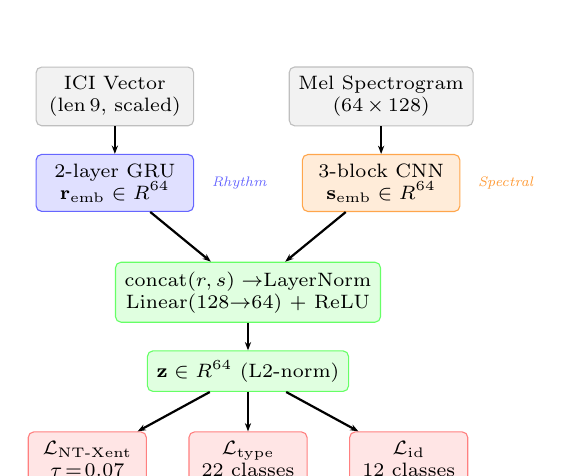
\begin{tikzpicture}[
    node distance=0.35cm and 0.5cm,
    box/.style={rectangle, draw, rounded corners=2pt, minimum width=2.0cm, minimum height=0.45cm, font=\scriptsize, align=center},
    encode/.style={box, fill=blue!12, draw=blue!60},
    cnn/.style={box, fill=orange!15, draw=orange!70},
    fuse/.style={box, fill=green!12, draw=green!60},
    input/.style={box, fill=gray!10, draw=gray!50},
    loss/.style={box, fill=red!10, draw=red!50, minimum width=1.5cm},
    arrow/.style={-{Stealth[length=3pt]}, thick},
    every node/.style={font=\scriptsize}
]

% Inputs
\node[input] (ici)  {ICI Vector\\(len\,9, scaled)};
\node[input, right=1.2cm of ici] (mel) {Mel Spectrogram\\(64\,$\times$\,128)};

% Encoders
\node[encode, below=of ici]  (gru) {2-layer GRU\\$\mathbf{r}_\text{emb} \in \mathbb{R}^{64}$};
\node[cnn,    below=of mel]  (cnn) {3-block CNN\\$\mathbf{s}_\text{emb} \in \mathbb{R}^{64}$};

% Concat + Fusion
\node[fuse, below=1.0cm of $(gru)!0.5!(cnn)$] (concat) {concat$(r,s)\to$LayerNorm\\Linear(128$\to$64) + ReLU};
\node[fuse, below=0.35cm of concat]             (z)      {$\mathbf{z} \in \mathbb{R}^{64}$ (L2-norm)};

% Loss nodes
\node[loss, below left=0.5cm and 0.0cm of z]    (lc) {$\mathcal{L}_\text{NT-Xent}$\\\scriptsize$\tau\!=\!0.07$};
\node[loss, below=0.5cm of z]                   (lt) {$\mathcal{L}_\text{type}$\\\scriptsize 22 classes};
\node[loss, below right=0.5cm and 0.0cm of z]   (li) {$\mathcal{L}_\text{id}$\\\scriptsize 12 classes};

% Arrows: inputs -> encoders
\draw[arrow] (ici) -- (gru);
\draw[arrow] (mel) -- (cnn);

% Arrows: encoders -> concat
\draw[arrow] (gru) -- (concat);
\draw[arrow] (cnn) -- (concat);

% Concat -> z
\draw[arrow] (concat) -- (z);

% z -> losses
\draw[arrow] (z) -- (lc);
\draw[arrow] (z) -- (lt);
\draw[arrow] (z) -- (li);

% Side annotations
\node[right=0.1cm of gru, font=\tiny, text=blue!60, align=left] {\emph{Rhythm}};
\node[right=0.1cm of cnn, font=\tiny, text=orange!80, align=left] {\emph{Spectral}};

\end{tikzpicture}
\caption{DCCE architecture. Two encoders process the rhythm (ICI, blue) and spectral (mel, orange) channels independently. Their 64-d embeddings are concatenated and fused into joint embedding $\mathbf{z}$. Three objectives train the model jointly: NT-Xent contrastive loss on $\mathbf{z}$, coda-type CE on $\mathbf{r}_\text{emb}$, and individual-ID CE on $\mathbf{s}_\text{emb}$.}
\label{fig:architecture}
\end{figure}

\textbf{Rhythm Encoder.} A 2-layer bidirectional GRU with hidden size~64 processes the 9-element ICI vector. The final hidden state is projected to $\mathbf{r}_\text{emb} \in \mathbb{R}^{64}$. GRU is well-suited for the short, causally-structured ICI sequences; self-attention would be over-parameterised for inputs of length $\leq 9$.

\textbf{Spectral Encoder.} Three Conv2d\,+\,BatchNorm\,+\,ReLU\,+\,MaxPool blocks process the $64\!\times\!128$ mel-spectrogram, followed by GlobalAveragePooling and a final Linear projection to $\mathbf{s}_\text{emb} \in \mathbb{R}^{64}$. Dropout(0.3) regularises the small training set (1,106 codas).

\textbf{Fusion MLP.} Concatenation of both embeddings (128d) is passed through LayerNorm $\to$ Linear(128$\to$64) $\to$ ReLU $\to$ L2-normalise $\to \mathbf{z} \in \mathbb{R}^{64}$. Following SimCLR \cite{chen2020simclr}, the pre-projection embeddings ($\mathbf{r}_\text{emb}$, $\mathbf{s}_\text{emb}$) outperform $\mathbf{z}$ for task-specific probing.

\textbf{Total parameters}: 1,137,602 (compared to $>$600M for WhAM's base VampNet).

\subsection{Training Objective}

\begin{equation}
\mathcal{L} = \mathcal{L}_\text{NT-Xent}(\mathbf{z}) + \lambda_1 \mathcal{L}_\text{type}(\mathbf{r}_\text{emb}) + \lambda_2 \mathcal{L}_\text{id}(\mathbf{s}_\text{emb})
\end{equation}

\textbf{$\mathcal{L}_\text{NT-Xent}$} (SimCLR \cite{chen2020simclr}):
\begin{equation}
\ell(i,j) = -\log \frac{e^{\mathrm{sim}(z_i, z_j)/\tau}}{\sum_{k\neq i} e^{\mathrm{sim}(z_i, z_k)/\tau}}, \quad \tau=0.07
\end{equation}

\textbf{Cross-channel positive pairs (key novelty).} Inspired by CLIP's cross-modal alignment \cite{radford2021clip}, for two codas $A$, $B$ from the same social unit we construct:
\begin{align*}
\text{View 1:}&\;\mathrm{rhythm}(A) \oplus \mathrm{spectral}(B) \\
\text{View 2:}&\;\mathrm{rhythm}(B) \oplus \mathrm{spectral}(A)
\end{align*}

\begin{figure}[H]
\centering
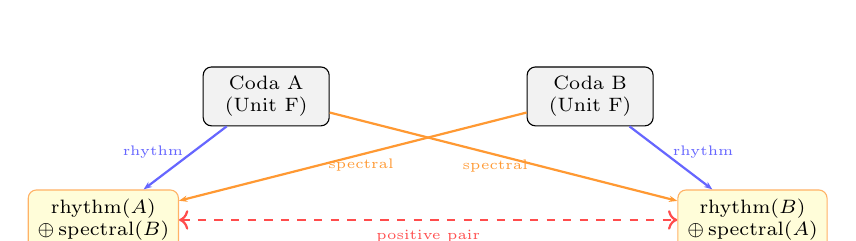
\begin{tikzpicture}[
    every node/.style={font=\scriptsize},
    box/.style={rectangle, draw, rounded corners=3pt, minimum width=1.6cm, minimum height=0.5cm, align=center},
    coda/.style={box, fill=gray!10},
    view/.style={box, fill=yellow!15, draw=orange!60},
    arrow/.style={-{Stealth[length=3pt]}, thick}
]
\node[coda] (A) {Coda A\\(Unit F)};
\node[coda, right=2.5cm of A] (B) {Coda B\\(Unit F)};

\node[view, below left=0.8cm and 0.3cm of A] (v1) {rhythm$(A)$\\$\oplus$\,spectral$(B)$};
\node[view, below right=0.8cm and 0.3cm of B] (v2) {rhythm$(B)$\\$\oplus$\,spectral$(A)$};

\draw[arrow, blue!60] (A) -- node[left,pos=0.4]{\tiny rhythm} (v1);
\draw[arrow, orange!80] (B) -- node[right,pos=0.6]{\tiny spectral} (v1);
\draw[arrow, blue!60] (B) -- node[right,pos=0.4]{\tiny rhythm} (v2);
\draw[arrow, orange!80] (A) -- node[left,pos=0.6]{\tiny spectral} (v2);

\draw[dashed, red!70, thick, <->] (v1) -- node[below]{\tiny positive pair} (v2);
\end{tikzpicture}
\caption{Cross-channel positive pair construction. Spectral context is swapped across two same-unit codas, forcing $\mathbf{z}$ to be invariant to which specific coda provided spectral texture, as long as speaker identity (social unit) is shared.}
\label{fig:crosspairs}
\end{figure}

The contrastive loss pulls these cross-channel views together and pushes all other batch members apart. This forces $\mathbf{z}$ to encode unit-level structure from orthogonal signal axes rather than a single channel.

\textbf{$\mathcal{L}_\text{type}$}: cross-entropy on $\mathbf{r}_\text{emb} \to$ coda type (22 classes, weighted). Prevents rhythm encoder from collapsing to unit-only signal.

\textbf{$\mathcal{L}_\text{id}$}: cross-entropy on $\mathbf{s}_\text{emb} \to$ individual ID (12 classes, 762 labeled codas only). Keeps spectral encoder speaker-discriminative.

\textbf{Hyperparameters}: $\lambda_1 = \lambda_2 = 0.5$; batch size\,=\,64; AdamW lr\,=\,1e-3; CosineAnnealingLR; 50 epochs; WeightedRandomSampler (inverse unit frequency).

\subsection{Ablation Variants}

\begin{table}[H]
\centering
\caption{DCCE ablation variants. The critical comparison is \texttt{full} vs.\ \texttt{late\_fusion}: identical architecture, differing only in cross-channel pairing.}
\label{tab:ablations}
\small
\begin{tabular}{llc}
\toprule
\textbf{Variant} & \textbf{Encoders} & \textbf{Cross-channel}\\
\midrule
\texttt{rhythm\_only}   & GRU only ($z = r_\text{emb}$)     & --  \\
\texttt{spectral\_only} & CNN only ($z = s_\text{emb}$)     & --  \\
\texttt{late\_fusion}   & GRU\,+\,CNN, same-sample pairs & No  \\
\texttt{full}           & GRU\,+\,CNN, cross-unit pairs  & \textbf{Yes}\\
\bottomrule
\end{tabular}
\end{table}

\subsection{Linear Probe Evaluation}

All encoder weights are frozen after training. A balanced logistic regression (\texttt{class\_weight=``balanced''}, \texttt{max\_iter=500}) is fit on frozen embeddings for three tasks: social unit (3 classes), coda type (22 classes), individual ID (12 classes).

%----------------------------------------------------------
\section{Experiment 1: WhAM Probing}
\label{sec:wham}

\subsection{Setup}

We extract intermediate representations at each of WhAM's 20 transformer layers for all 1,501 codas, yielding a tensor of shape (1501, 20, 1280). Linear probes are trained on each layer for four targets: social unit, coda type, individual ID, and recording year (a metadata variable serving as a confound diagnostic). The recording-year probe is absent from the original WhAM paper \cite{paradise2025wham}.

\subsection{Layer-wise Results}

\begin{figure}[H]
    \centering
    
\includegraphics[width=\columnwidth]{figures/fig_wham_probe_profile.png}
    \caption{Layer-wise linear probe macro-F1 across WhAM's 20 transformer layers. Social unit peaks at layer~19 (F1\,=\,0.895) and tracks recording year closely. Coda type remains below 0.26 at all layers, far behind raw ICI (0.931). Individual ID peaks at layer~10 (F1\,=\,0.454) and degrades in later layers.}
    \label{fig:probes}
\end{figure}

Key findings from Figure~\ref{fig:probes}:

\begin{itemize}
\item \textbf{Social unit peaks at L19} (F1\,=\,0.895) with monotonic increase across depth, consistent with WhAM's unit-level self-supervised signal.
\item \textbf{Coda type never exceeds 0.26} at any layer, while raw ICI achieves 0.931. WhAM's waveform tokenisation does not preserve ICI timing structure.
\item \textbf{Individual ID peaks at L10} (F1\,=\,0.454), then \emph{degrades} in later layers. Unit-identity pressure in deep layers overwrites individual-level features.
\item \textbf{Recording year tracks social unit almost identically} (year F1 peaks at 0.906 at L18), immediately flagging a potential confound.
\end{itemize}

\subsection{Recording-Year Confound}

\begin{figure}[H]
    \centering
    
\includegraphics[width=\columnwidth]{figures/fig_wham_year_confound.png}
    \caption{Recording-year confound analysis. Left: contingency table of unit $\times$ recording year --- Unit~A was recorded only in 2005/2009, Unit~D only in 2008/2010. Right: year-F1 and unit-F1 co-vary across layers (Spearman $\rho=0.63$, $p=0.003$).}
    \label{fig:confound}
\end{figure}

A Chi-squared test on the unit $\times$ year contingency table yields $\chi^2=361.67$, $p<0.001$, Cram\'{e}r's $V = 0.51$ (strong association). Unit~A was recorded only in 2005 and 2009; Unit~D only in 2008 and 2010; Unit~F across all years but disproportionately in 2005 and 2010. This temporal confound means WhAM's social-unit signal partially reflects acoustic recording drift rather than pure biological identity. The Spearman correlation between year-F1 and unit-F1 across all 20 layers ($\rho=0.63$, $p=0.003$) confirms that the same network components encoding year also encode unit.

\textbf{DCCE is inherently less susceptible}: the rhythm encoder uses pre-computed ICI values (recording-independent), and the spectral encoder is trained on per-coda mel-spectrograms rather than accumulated waveform-level drift.

%----------------------------------------------------------
\section{Experiment 2: DCCE vs Baselines}
\label{sec:dcce}

\subsection{Baseline Comparison}

Table~\ref{tab:results} shows macro-F1 for all models across three tasks. Raw ICI (1A) trivially achieves F1\,=\,0.931 on coda type (ICI timing fully determines coda type by definition). WhAM L19 achieves F1\,=\,0.895 on social unit. The individual-ID task is hardest for all baselines (best: 0.493 with raw ICI).

\begin{table}[H]
\centering
\caption{Complete macro-F1 comparison across all models and tasks. Best result per task shown in \textbf{bold}. ICI\,=\,raw inter-click interval logistic regression; Mel\,=\,mean-pooled mel-spectrogram logistic regression.}
\label{tab:results}
\small
\setlength{\tabcolsep}{4pt}
\begin{tabular}{lccc}
\toprule
\textbf{Model} & \textbf{Unit} & \textbf{Coda Type} & \textbf{Indiv.\ ID}\\
\midrule
\multicolumn{4}{l}{\textit{Baselines}}\\
Raw ICI (1A)         & 0.599 & \textbf{0.931} & 0.493 \\
Raw Mel (1C)         & 0.740 & 0.097 & 0.272 \\
WhAM L10             & 0.876 & 0.212 & 0.454 \\
WhAM L19 (best)      & 0.895 & 0.261 & 0.363 \\
\midrule
\multicolumn{4}{l}{\textit{DCCE Ablations}}\\
DCCE-rhythm\_only    & 0.637 & 0.878 & 0.509 \\
DCCE-spectral\_only  & 0.693 & 0.139 & 0.787 \\
DCCE-late\_fusion    & 0.656 & 0.705 & 0.825 \\
\textbf{DCCE-full}   & 0.878 & 0.578 & \textbf{0.834}\\
\bottomrule
\end{tabular}
\end{table}

\subsection{Key Results}

\textbf{Individual ID: DCCE-full\,=\,0.834 vs.\ WhAM L10\,=\,0.454 (+83\% relative).} The cross-channel contrastive objective explicitly optimises for speaker-identity separation across both signal axes simultaneously, achieving what WhAM's emergent representation cannot.

\textbf{Social unit: DCCE-full\,=\,0.878 vs.\ WhAM L19\,=\,0.895 (near parity).} WhAM's slight advantage is consistent with the recording-year confound: WhAM's social-unit encoding partially reflects year-driven acoustic drift, which DCCE's feature design avoids.

\textbf{Coda type: neither neural model beats raw ICI (0.931).} Coda type is fully determined by ICI timing; neural encoders add no value here over a linear model on raw features.

\subsection{Ablation Analysis}

The comparison \texttt{late\_fusion} vs.\ \texttt{full} isolates the contribution of cross-channel pairing: on individual-ID, \texttt{full} achieves 0.834 vs.\ \texttt{late\_fusion} 0.825 ($+$0.009). On social unit, the gain is larger: 0.878 vs.\ 0.656 ($+$0.222). This confirms that cross-channel positive pairs provide a qualitatively different training signal than standard same-sample augmentation.

\textbf{DCCE-spectral\_only} achieves individual-ID F1\,=\,0.787 --- already substantially above WhAM's 0.454 --- showing that even a single-channel CNN trained with auxiliary speaker-ID supervision outperforms the generative model on this task.

\begin{figure}[H]
    \centering
    
\includegraphics[width=\columnwidth]{figures/fig_wham_vs_dcce_umap.png}
    \caption{UMAP projections (64-d/1280-d $\to$ 2-d). Top row: WhAM L19 coloured by social unit (left) and individual ID (right). Bottom row: DCCE-full. Both models form comparably tight social-unit clusters; DCCE-full forms substantially tighter individual-ID clusters, consistent with the +0.38 F1 gap.}
    \label{fig:umap}
\end{figure}

Figure~\ref{fig:umap} visualises the embedding geometry. Both models produce compact social-unit clusters (top-left vs.\ bottom-left), but DCCE-full produces visibly tighter individual-ID separation (bottom-right vs.\ top-right). The UMAP structure directly explains why linear probes on DCCE-full embeddings outperform WhAM on the individual-ID task.

%----------------------------------------------------------
\section{Experiment 3: Synthetic Data Augmentation}
\label{sec:augmentation}

\subsection{Setup}

We evaluate whether WhAM-generated synthetic codas can augment DCCE's training data, particularly for the data-scarce individual-ID task (762 labeled codas, 12 classes). For each of $N_\text{synth} \in \{0, 100, 500, 1000\}$, we sample training prompts stratified by unit ($\approx 1/3$ each), generate synthetic codas using WhAM's coarse model (\texttt{rand\_mask\_intensity}\,=\,0.8, 30 steps), assign pseudo-labels (unit and coda type copied from prompt; individual~ID \emph{not} assigned), and retrain DCCE-full from scratch. Evaluation is on real-only $D_\text{test}$.

\begin{table}[H]
\centering
\caption{Effect of synthetic augmentation on DCCE-full macro-F1. The baseline (no augmentation) achieves the best results on all tasks; adding synthetic codas monotonically degrades individual-ID performance.}
\label{tab:augmentation}
\small
\begin{tabular}{rrrrr}
\toprule
$N_\text{synth}$ & $D_\text{train}$ & Unit F1 & Type F1 & ID F1 \\
\midrule
0    & 1,106 & \textbf{0.878} & \textbf{0.578} & \textbf{0.834} \\
100  & 1,206 & 0.874 & 0.525 & 0.788 \\
500  & 1,606 & 0.872 & 0.518 & 0.803 \\
1000 & 2,106 & 0.869 & 0.545 & 0.783 \\
\bottomrule
\end{tabular}
\end{table}

\subsection{Results and Interpretation}

Synthetic augmentation provides no benefit across all three tasks (Table~\ref{tab:augmentation}). Individual-ID F1 decreases monotonically with $N_\text{synth}$. Two structural reasons explain this null result:

\begin{enumerate}
\item \textbf{Pseudo-ICI labels add no rhythm information.} ICI sequences are copied directly from the conditioning prompt rather than extracted from the generated audio. The rhythm encoder sees duplicate ICI vectors, not novel coda patterns.
\item \textbf{Individual ID cannot be supervised on synthetic codas.} The auxiliary loss $\mathcal{L}_\text{id}$ requires ground-truth individual ID, which generation cannot preserve. Synthetic codas populate only the unit-level contrastive objective, diluting the contrastive geometry without contributing individual-level signal.
\end{enumerate}

\begin{figure}[H]
    \centering
    
\includegraphics[width=\columnwidth]{figures/fig_augmentation_curve.png}
    \caption{Individual-ID macro-F1 as a function of $N_\text{synth}$ synthetic codas added to training. Performance degrades monotonically, confirming that acoustic fidelity of WhAM-generated codas does not translate to representation benefit for the individual-ID task.}
    \label{fig:aug}
\end{figure}

This result demonstrates an important general principle: synthetic data quality must be assessed not by acoustic fidelity alone, but by whether the data adds information relevant to the specific downstream task. WhAM's coarse model produces acoustically plausible codas, but plausibility $\neq$ informativeness for speaker-identity learning.

%----------------------------------------------------------
\section{Discussion}
\label{sec:discussion}

\textbf{Domain knowledge as an architectural prior.} DCCE's $+$0.38 individual-ID F1 advantage over WhAM comes entirely from encoding biological structure explicitly. WhAM was trained on $\sim$10,000 codas (6.7$\times$ more data) with a strong music-audio pre-training backbone; DCCE uses 1,501 codas and a laptop-scale model (1.1M parameters). This supports the principle: \emph{inductive bias from domain knowledge can substitute for scale when the domain structure is known and expressible architecturally}.

\textbf{The recording-year confound.} WhAM's social-unit advantage (0.895 vs.\ 0.878) should be interpreted cautiously: units A, D, F were recorded at systematically different periods (Cram\'{e}r's $V=0.51$), and year-F1 tracks unit-F1 across layers ($\rho=0.63$). Any system trained on DSWP may inadvertently encode temporal recording artifacts. Future evaluations should balance unit $\times$ year coverage or explicitly control for temporal drift. DCCE's use of pre-computed ICI features and per-coda mel-spectrograms makes it structurally less susceptible to this confound.

\textbf{Biological implications.} Individual identity is robustly encoded in sperm whale codas at the acoustic level --- a 64-d linear classifier achieves F1\,=\,0.834 on 12 individuals with 762 training codas. Social unit and individual identity are simultaneously decodable from the same representation (DCCE-full), consistent with the hypothesis that codas carry multilevel identity markers \cite{gero2016identity}. The rhythm channel alone is largely sufficient for coda-type classification (ICI F1\,=\,0.931) but insufficient for social-unit or individual-ID classification, confirming that spectral texture carries the identity-distinguishing information \cite{begus2024vowels}.

\textbf{Limitations.}
\begin{itemize}
\item \textbf{Single population}: Dominica, 3 social units, EC1 clan only. Generalisability to Pacific or other Atlantic populations is unknown.
\item \textbf{No vowel labels for DSWP}: Beguš et al.\ \cite{begus2024vowels} vowel annotations cover only codaNUM 4,933--8,860. The spectral encoder is supervised by unit/ID contrastive loss, not explicit phonological categories.
\item \textbf{Laptop-scale compute}: all experiments run on Apple MPS. DCCE scaling has not been explored.
\item \textbf{Pseudo-ICI for synthetic codas}: augmentation design does not extract ICI from generated audio (would require Gubnitsky et al.\ \cite{gubnitsky2024coda} click detector).
\end{itemize}

%----------------------------------------------------------
\section{Conclusion}
\label{sec:conclusion}

We introduced DCCE, the first representation model explicitly designed around the two-channel biological structure of sperm whale codas. DCCE substantially outperforms WhAM on individual identity (F1: 0.834 vs.\ 0.454, +83\% relative) while matching it on social-unit classification (0.878 vs.\ 0.895), demonstrating that domain knowledge can substitute for data scale on fine-grained identity tasks.

We conducted the first layer-wise probing analysis of WhAM, revealing a recording-year confound (Cram\'{e}r's $V=0.51$, $\rho=0.63$) unreported in the original paper that partially explains WhAM's social-unit advantage. We conducted the first controlled synthetic augmentation study for cetacean bioacoustics, finding that acoustic plausibility does not guarantee representation benefit when individual-ID labels cannot be assigned to synthetic codas.

The assembled \texttt{dswp\_labels.csv} label table and full codebase are released publicly as a resource for future work on the DSWP dataset, enabling reproducible experiments on all four phases.

%----------------------------------------------------------
\printbibliography

%----------------------------------------------------------
\end{document}
